\subsection{Manual Energy Correction in \p0d}
\label{sec:EnergyCorrection}

A MC particle gun study on the \p0d energy reconstruction systematic 
showed that a large fraction (approximately $10$\%) of globalRecon
reconstructed events were significantly shifted from the true momentum, causing a 
secondary peak structure.  This effect is due to a known bug in the Spin-C and 
Spin-D global reconstruction when the SMRD is used.  For the purposes of this 
study, we had two clear solutions until the next ND280 software processing: $1)$
cut out all SMRD used tracks, or $2)$ do a manual energy loss correction using
TPC1 momentum.  This section describes the second approach.

To speed up the energy loss correction, we 
did not use the
$\frac{dE}{dx}$ tables and incrementally adjust the energy.  Instead, 
the \p0d energy loss was calculated using range data for the various superP0Dules.
Range is defined here as $R(E')=\int^{E'}_0 \left(\frac{dE}{dx}\right)^{-1}\,dE$, where
$\frac{dE}{dx}$ is the weighted average over all materials, and is calculated for each superP0Dule.  
This gave us a table of range vs energy/momentum for every part of the \p0d and 
essentially allowed us to perform the integration once as opposed to 
doing this repeatedly for every track.
To obtain the energy lost in the \p0d, we simply take the TPC1 momentum, find its 
corresponding range, add the length of the track in next superP0Dule, and find
the corresponding momentum (see figure \ref{fig:energyCorr}).  We repeat this as 
necessary depending on whether the track traversed through more than one superP0Dule.

This correction fixes the momenta of all tracks which used the SMRD.
Furthermore, it appears to agree well with the the global front momentum for tracks which
do not use the SMRD. In Figure \ref{fig:correctedECompare})
the corrected values are compared to the MC truth values and good agreement
is obtained.  Consequently, it is 
effective for both correcting tracks with the SMRD bug, as well as for an independent
 analysis involving only the \p0d and TPC1.

\begin{figure}
\centering
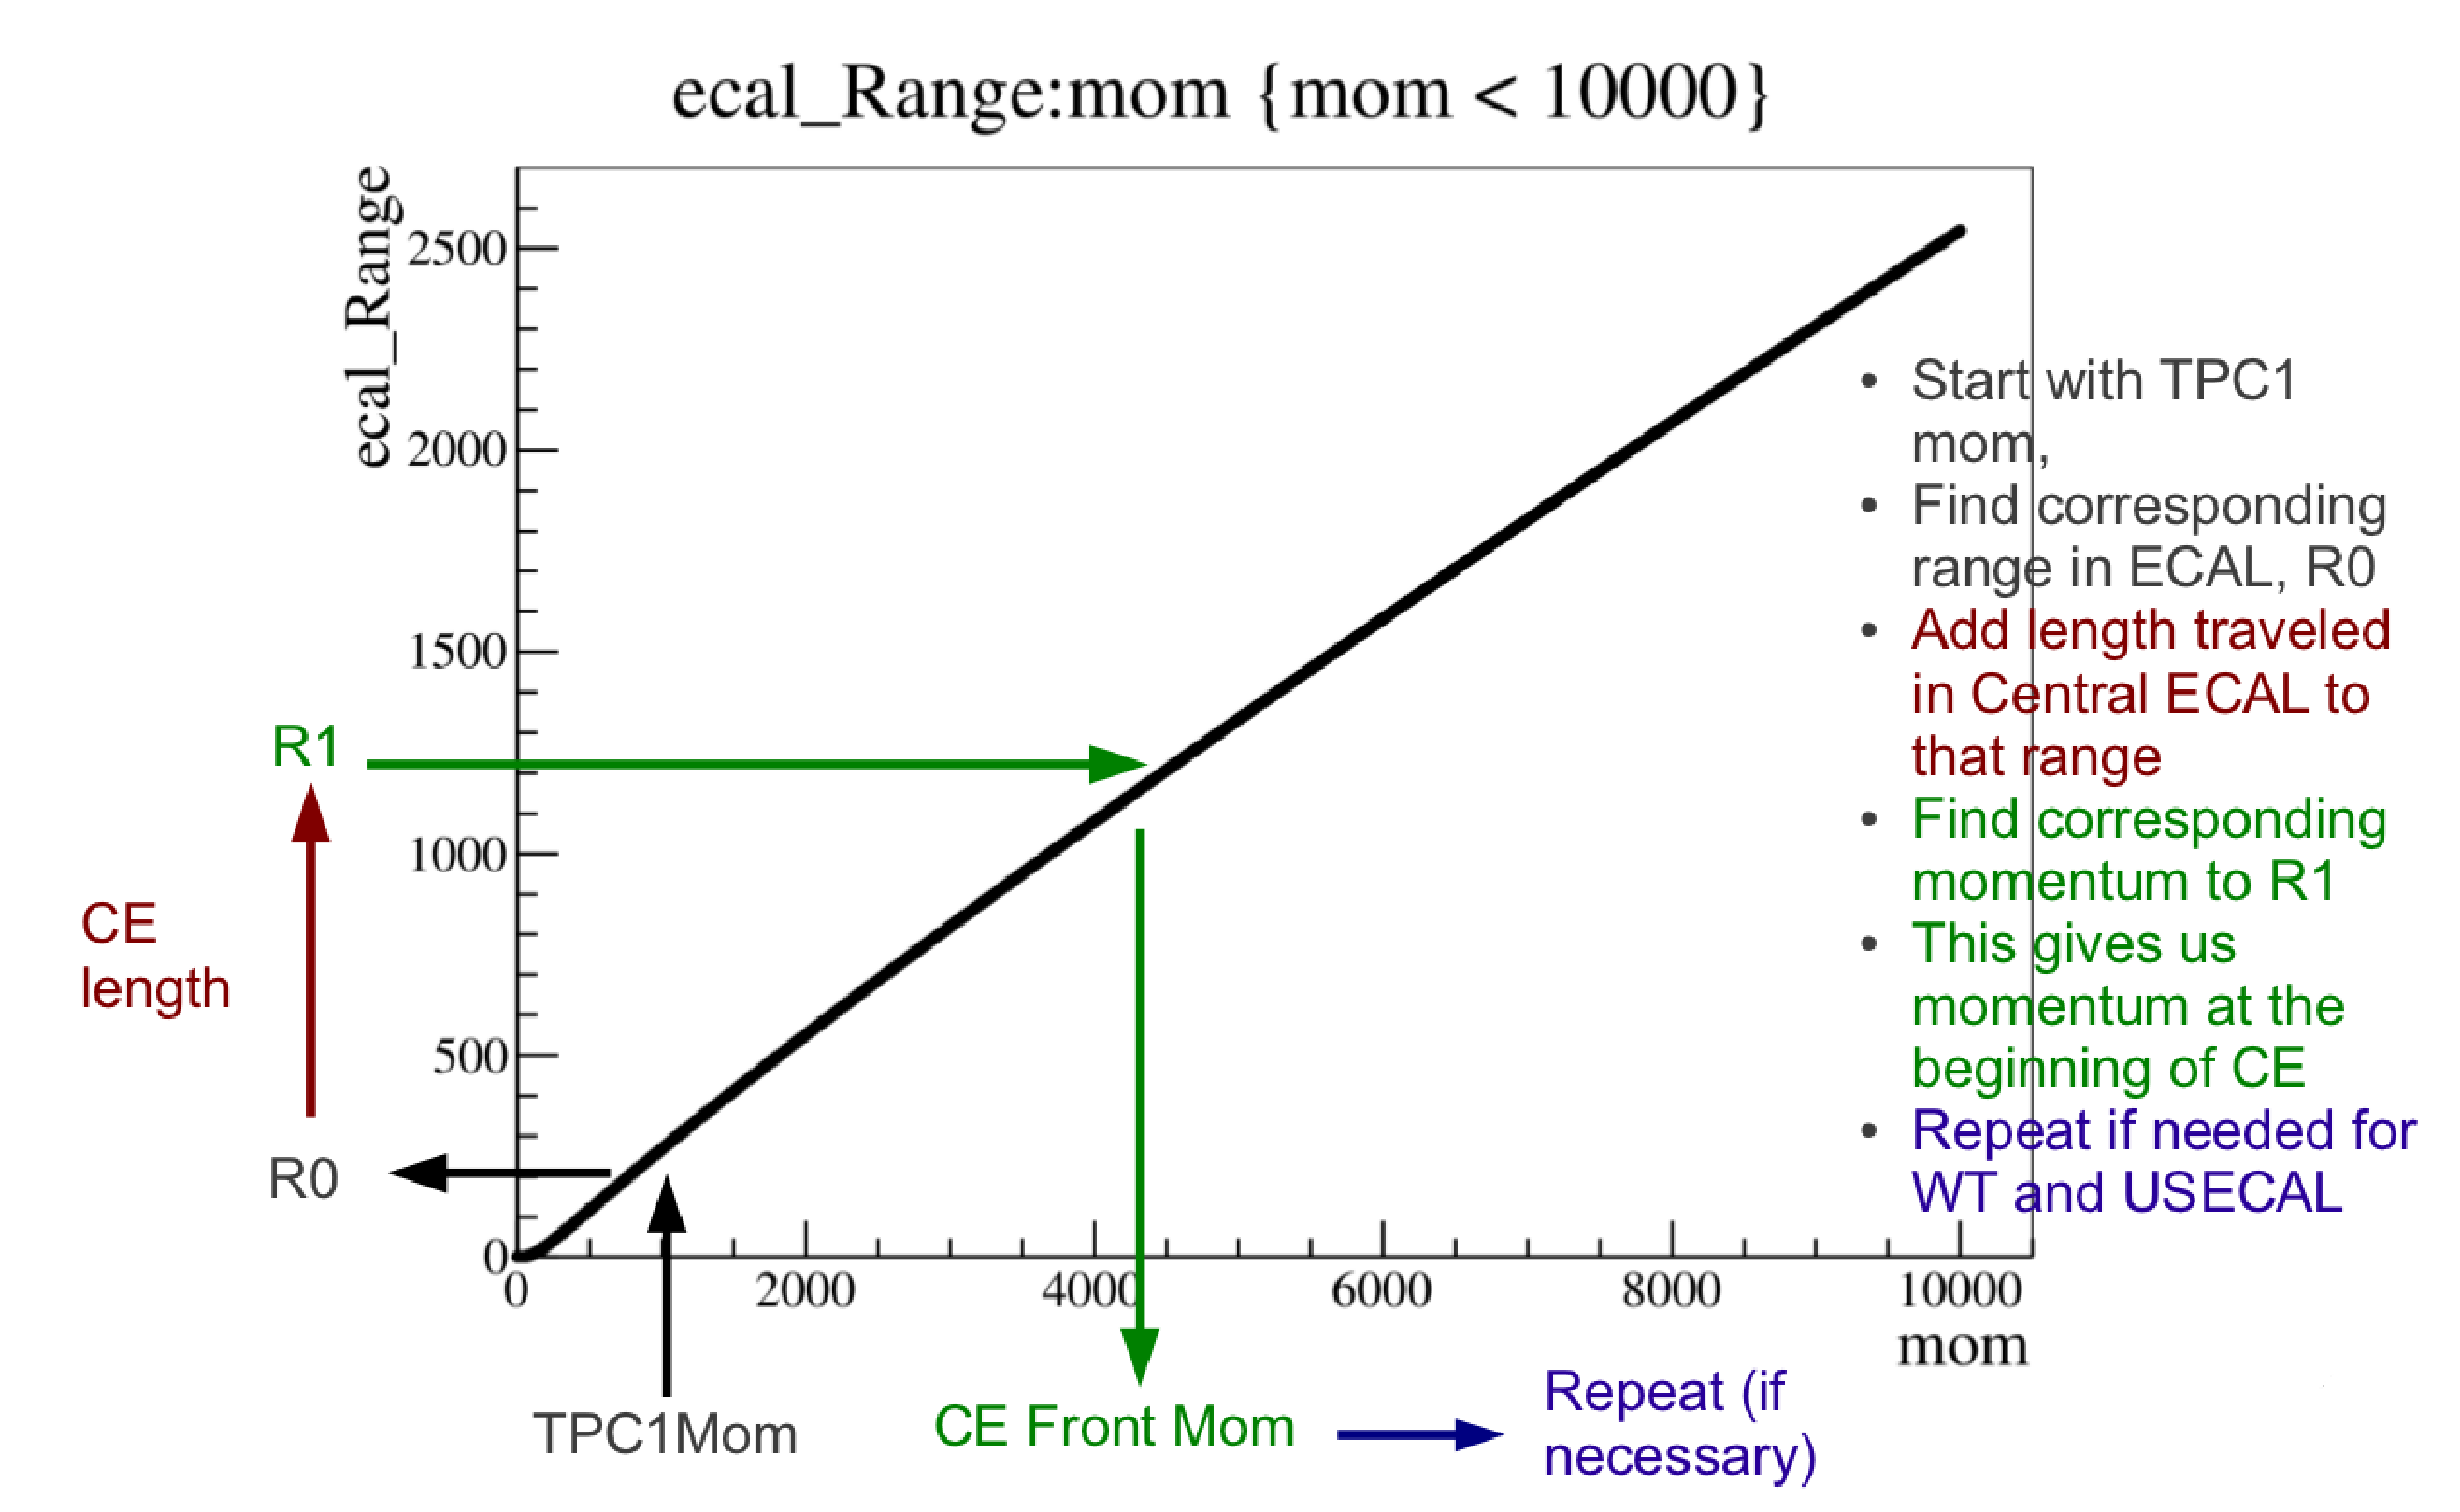
\includegraphics[width=5.5in]{Figures/eLossCalc1.eps}
\caption{Calculation of \p0d momentum correction. The steps of the correction
are schematically shown with the arrows} 
\label{fig:energyCorr}
\end{figure}

\begin{figure}
\centering
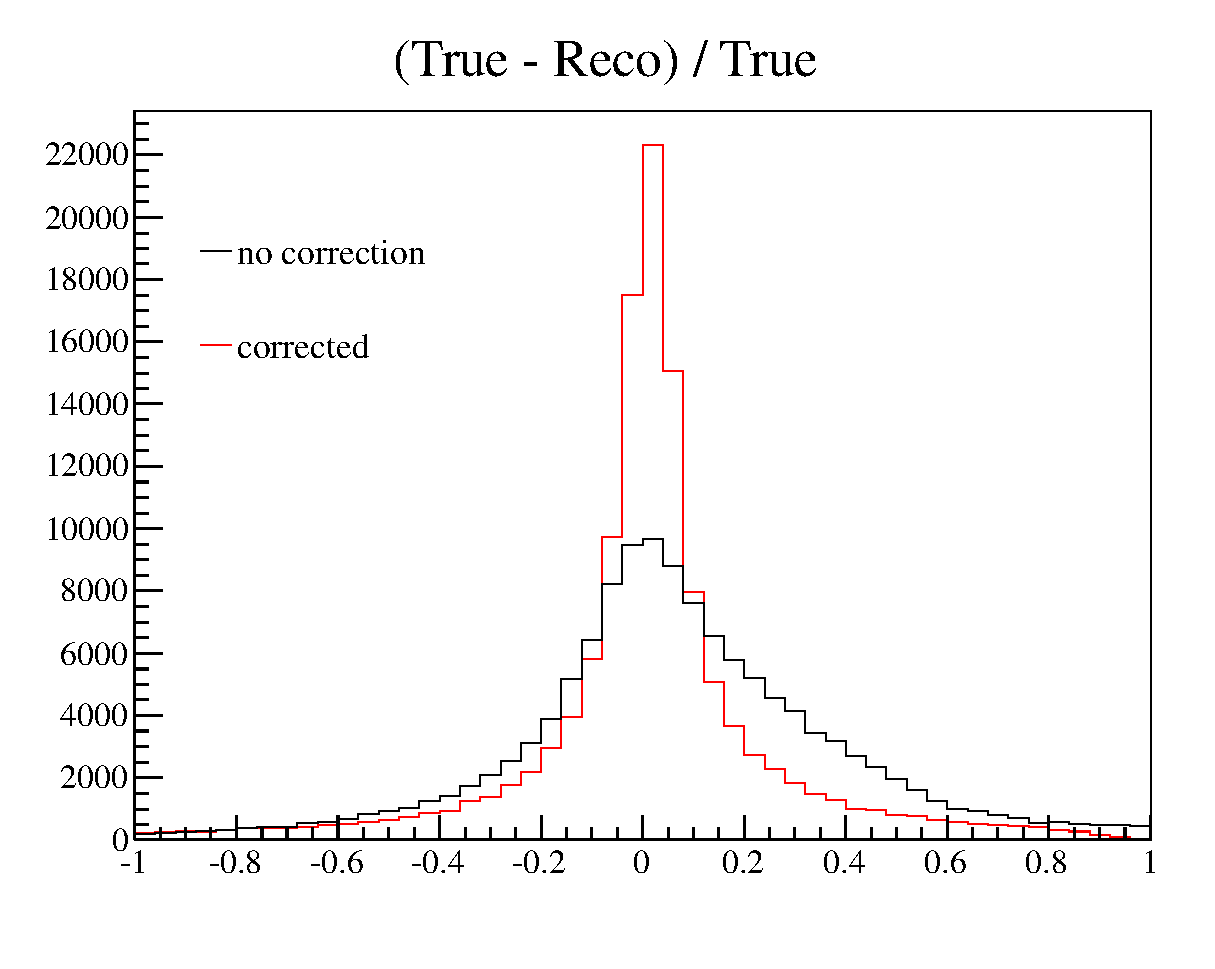
\includegraphics[width=5.5in]{Figures/eCompare.eps}
\caption{Comparison of mcp4C globalRecon \p0d momenta (black) vs manually corrected \p0d momenta (red).  Note that 
the manually corrected momenta are closer to the true momenta than globalRecon.} 
\label{fig:correctedECompare}
\end{figure}
